\chapter{Evaluation}
\label{chap:evaluation}

\section{What is Ragas?}
Ragas is an evaluation framework for retrieval-augmented generation. It measures the quality of generated answers against their retrieved context. In this project, the principal metrics are faithfulness, answer relevancy and context precision. Faithfulness checks whether the answer is supported by the context; answer relevancy checks whether it addresses the question; and context precision checks whether the retrieved passages are useful and well-ranked.

\section{Retrieval Evaluation}
The current reviewed evaluation contains 39 documents, 534 chunks and 4 questions. Vector retrieval and GraphRAG both achieved Recall@5 of 0.75, MRR of 0.5833 and nDCG@5 of 0.625. Mean latency was 74.36 ms for vector retrieval and 94.32 ms for GraphRAG. The result is a tie: on this small corpus, the graph contributes explainability and provenance rather than a measured ranking advantage.

\begin{figure}[H]
\centering
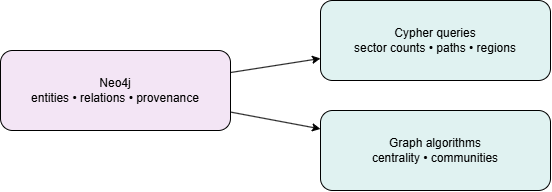
\includegraphics[width=0.9\textwidth]{images/04-neo4j-analytics.png}
\caption{Knowledge-graph storage and analytics view.}
\label{fig:graph-analytics}
\end{figure}

\section{Ragas Results}
Ragas execution is wired through \texttt{scripts/evaluate\_ragas.py} and its results are exposed by the FastAPI \texttt{/evaluation} endpoint. The frontend displays faithfulness, answer relevancy and context precision when \texttt{data/ragas\_results.json} is available. Scores must be generated with valid provider credentials; missing scores are not presented as successful results.

\section{Data Quality Statistics}
The source-quality checker currently reports an average score of \textbf{76.6/100}. It combines authority, provenance, completeness and freshness. The corpus is therefore suitable for a functional demonstration, but the score is a provenance heuristic rather than a human-annotated truth-quality measure.

\section{Interpretation and Limits}
The retrieval cases are reviewed external cases, but the corpus remains small. Ragas scores should therefore be interpreted as an initial quality signal, not as a generalization guarantee. A larger reviewed Arabic/French question set and repeated provider-controlled runs are required for a final benchmark.
